\chapter{Présentation du stage}

\section{Le sujet}
\label{le-sujet}
Le sujet du stage était initialement \enquote{\textit{Developer C++/Qt.
work on a challenging and immersive 360 video software}}.\\
Bien que le sujet soit assez général, le domaine de l'entreprise se trouvait être très intéressant
et durant l'entretien qui s'est déroulé à la mi-mai, quelques sujets ont été
abordés~: Nicolas Burtey a proposé de travailler sur le VideoStitch Player d'une part,
à la suite d'Alexis Pontin et pour terminer son travail, et d'autre part de
travailler au développement du nouveau produit,
Vahana VR, qui allait débuter dans quelques semaines.\\
M. Burtey n'était pas encore certain de développer Vahana VR, 
et envisageait également à la conception du \textit{stitch} stéréoscopique 3D\footnote{Qui
consiste, brièvement, en la conception de deux équirectangulaires pour la même
scène filmée~: un pour chaque œil en exploitant l'effet de la parallaxe, recréant 
un effet de relief\cite{videostitch-stereo}
\cite{image-stereoscopique}}~: il proposa également un sujet sur 
la prise en charge de la 360 stéréo dans Videostitch Studio.\\
Le sujet final serait décidé la première semaine du stage.\\
\newline
Le stage fut finalement précédé par un CDD, les missions retenues
se sont alors simplement étendues du début du CDD à la fin du stage.\\
Le sujet réel a donc été arrêté à deux missions~:
\begin{enumerate}
  \item Simplifier et améliorer le \textit{workflow} de développement, d'une
  gestion mono-logicielle vers une gestion multi-logicielle, en y intégrant 
  le VideoStitch Player et Vahana VR.
  \item Développer et le déployer un système de \textit{plugins} basés
  sur des caméras et des cartes d'acquisitions, et augmentant les
  capacités entrées/sorties de Vahana VR.
\end{enumerate}
Ces deux missions\footnote{La 3D s'est révélée être 
une tâche trop ardue, après un rapide état de l'art du sujet par les ingénieurs~: 
même si les articles de recherche et brevets sont nombreux, aucune application 
industrielle n'a encore aujourd'hui aboutis.} trouvent comme sujet commun \emph{l'amélioration et la conception 
de \textit{workflows} à l'usage de l'équipe de développement}. La première consiste en 
ce sens à l'amélioration du système de développement et des outils qui y sont associés ainsi qu'à l'intégration des logiciels
de l'entreprise. La seconde permet, elle, par un système indépendant et modulaire, d'apporter
nouvelles capacités à Vahana VR, qui seront utilisées par les ingénieurs pour le développement de ce logiciel.

\section{Les méthodes de travail}
Le travail de l'équipe des développeurs s'appuie en grande partie sur la méthode \emph{Scrum}, et
sur quelques pratiques de qualité logicielle issues de l'\textit{Extreme Programming}, comme l'intégration continue.
Ces deux méthodes sont des \emph{méthodologies agiles}\cite{methode-agile}.\\
\newline
Scrum présente un certain nombres de pratiques; les éléments utilisés 
dans le cadre de VideoStitch sont essentiellement des événements et des artefacts 
décrits dans le\textit{Scrum guide}\cite{scrum-guide}~:
\begin{itemize}
  \item \textbf{Sprint}~: le principe de la méthode repose sur le découpage du projet en 
	périodes de temps, nommées \emph{sprint}, dont la durée à VideoStitch fut de 
	une ou deux semaines selon les besoins. Chaque sprint possède un but à accomplir 
	durant la période allouée, ce qui permet une grande réactivité sur les besoins 
	du projet, qui est, dans le cas de VideoStitch, l'entreprise elle-même.
	\item \textbf{Scrum meeting}~: réunion qui marque la fin d'un sprint et permet la préparation 
	du suivant. Elle se déroule en trois temps~:
	\begin{enumerate}
		\item \textit{Revue du sprint}~: c'est un passage en revue de ce qui a été réalisé
		et de ce qui ne l'a pas été durant le sprint, ainsi qu'une démonstration 
		de ce qui a été complété. Cela permet de valider l'objectif et d'ajuster 
		la planification du projet en fonction de son avancement.
		\item \textit{Retrospective du sprint}~: elle a pour but une amélioration continue 
		de l'environnement de travail et des méthodes utilisées. Chacun peut proposer
		des éléments d'amélioration, qui après vote, seront mis en place dès le sprint
		suivant.
		\item \textit{Planification du sprint suivant}~: l'équipe détermine le but du sprint
		suivant, et à partir du \textit{backlog} en détermine son contenu concret en liste de tâches.
	\end{enumerate}
  \item \textbf{Backlog}~: c'est une liste de l'ensemble des tâches (appelées \emph{tickets})
  de tout ce qui est nécessaire pour enrichir le projet. Elle initialement créée avant
  le début du projet, et enrichie lors des sprints en fonction de l'apparition des besoins nouveaux.
  \item \textbf{Statuts des tickets}~: après être choisis du backlog au sprint courant, 
  un ticket doit passer trois statuts pour être considéré comme réalisé~:
    \begin{enumerate}
      \item \textit{Selected for development}~: le ticket n'est pas réalisée.
      \item \textit{In progress}~: le ticket est en cours de réalisation par un développeur.
      \item \textit{QA}~: le ticket est réalisé et attends une validation d'une autre personne.
      \item \textit{Done}~: le ticket est réalisé et validé. 
    \end{enumerate}
  \item \textbf{Stand-up}~: \label{stand-up} ou encore \textit{daily scrum}, est une courte réunion de 15 minutes
  se déroulant chaque matin pour faire le point entre tous les membres de l'équipe.
  Chacun aborde ce qu'il a effectué la veille, les difficultés éventuelles qu'il
  a rencontré et ce qu'il compte réaliser aujourd'hui pour atteindre l'objet du sprint.
\end{itemize}
\begin{figure}
  \centering
  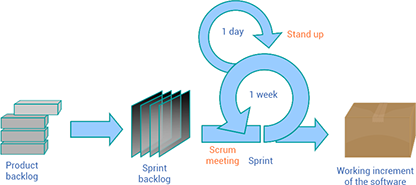
\includegraphics[width=11cm]{images/scrum-process.png}
  \caption{Illustration de la méthode Scrum\cite{scrum-process}}
\end{figure}
\ \newline
Cependant, le VideoStitch SDK et les ingénieurs y travaillant ne participent pas
aux sprints~: leur travail étant plutôt organisés sous formes de missions individuelles,
en fonction des besoins des applications de l'entreprise. Ils participent toutefois 
aux \textit{stand-up} et au \textit{retrospectives}.\\
Le présent stage a suivi l'équipe dans ses sprints, en l'assistant parfois sur quelques
tickets, tout en maintenant en priorité les deux missions de fond présentées plus haut, dans 
la section \cf{le-sujet}.\\
\newline
Enfin, toutes les communications écrites et orales se font en anglais, du fait
de la présence dans l'équipe de personnes de langue natale espagnole, allemande ou flamande.

\section{Les outils utilisés}
\label{outils-utilisés}
\paragraph{}
Les quatre produits de VideoStitch sont codés en \emph{C++}, avec utilisation des dernières possibilités
de C++11; VideoStitch SDK utilise également la bibliothèque \emph{CUDA} pour les calculs intensifs et parallélisables.
Le compilateur de chaque OS est utilisé~: g++ pour Linux, clang pour Max OS X et 
cl du Windows SDK, également utilisé par Visual Studio.
\paragraph{}
\begin{wrapfigure}[7]{l}{2.5cm}
  \centering
  
\includegraphics[width=2cm]{images/qt-logo.png}
  \caption{Logo de Qt}
\end{wrapfigure}
Les trois applications sont  
développées avec le framework C++ \emph{Qt}, qui permet d'assurer la portabilité sur les 
plateformes Windows, Linux et Mac OS X du même code source. En outre, Qt
propose un certain nombre de classes, en addition de la STL de C++, facilitant le
développement d'applications de haut niveau. Enfin ce framework est connu pour son
système de signals/slots ouvrant la voie à la programmation événementielle, et
asynchrone~: en addition à l'appel de fonctions, telle qu'existant depuis le C,
un objet peut émettre des \textit{signaux}. D'autres objets peuvent recevoir à leur tour
ces signaux pour exécuter des fonctions, appelées dans ce cas \textit{slot}.\cite{qt}
\paragraph{}
\begin{wrapfigure}[5]{r}{3.5cm}
  \centering
  
\includegraphics[width=3cm]{images/git-logo.png}
  \caption{Logo de Git}
\end{wrapfigure}
Tous les codes sources sont partagés et versionnés grâce au système de gestion de version 
distribué \emph{Git}\cite{gestion-versions}. Ce logiciel permet à l'équipe de travailler
avec des \emph{dépôts}~: un dépôt Git est simplement un dossier associé à une base
de donnée archivant l'historique de toutes les modifications qui y ont été effectuées. Chaque développeur
possède une copie de ce dépôt et de l'historique associé sur son ordinateur. Les développeurs se
transmettent régulièrement les modifications qu'ils ont apportées pour synchroniser
les historiques de toutes les copies~: ainsi, chaque membre de l'équipe sait qui a modifié quoi et quand.\\
En pratique, comme le montre la figure~\ref{git-diagram}, un serveur est utilisé pour sauvegarder les modifications faites en
servant de pont entre les développeurs~: chacun y propose ses modifications et l'interroge
sur les modifications des autres.
\paragraph{}
\begin{wrapfigure}[7]{l}{2.5cm}
  \centering
  
\includegraphics[width=1.5cm]{images/buildbot-logo.png}
  \caption{Logo de Buildbot}
\end{wrapfigure}
Enfin, à chaque modification apportée sur un dépôt Git, un serveur \emph{Buildbot} va exécuter
une routine, comme le montre la figure~\ref{buildbot-diagram}~: le produit concerné par la modification sera
compilé, subira un ensemble de tests de qualité et son installateur sera généré 
et mis à disposition sur une page de téléchargement à usage interne.\\
Ces installateurs pourront être utilisés par n'importe quelle personne de l'entreprise
pour des tests, en compléments avec les tests automatiques de qualité, pratique d'\emph{intégration continue},
qui permettent de vérifier à chaque modification effectuée qu'aucun bug, ni régression n'a été 
introduit\cite{integration-continue}.
\begin{figure}
  \centering
  \begin{minipage}[b]{0.4\textwidth}
    \centering
    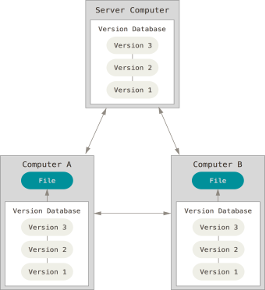
\includegraphics[width=7cm]{images/git-diagram.png}
    \caption{Schéma de gestion de version distribué\cite{pro-git}}
    \label{git-diagram}
  \end{minipage}%
  \hspace{0.09\textwidth}
  \begin{minipage}[b]{0.4\textwidth}
    \centering
    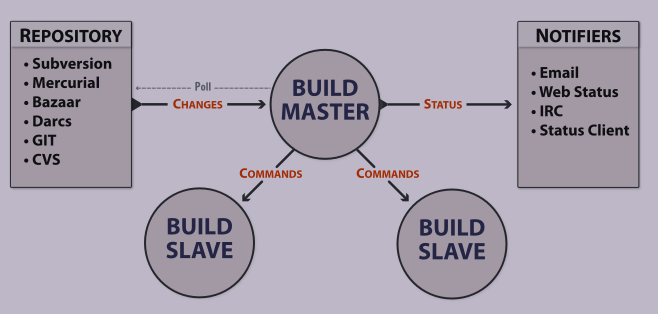
\includegraphics[width=7cm]{images/buildbot-diagram.png}
    \caption{Schéma de fonctionnement de Buildbot\cite{buildbot}}
    \label{buildbot-diagram}
  \end{minipage}
\end{figure}

